% Options for packages loaded elsewhere
% Options for packages loaded elsewhere
\PassOptionsToPackage{unicode}{hyperref}
\PassOptionsToPackage{hyphens}{url}
\PassOptionsToPackage{dvipsnames,svgnames,x11names}{xcolor}
%
\documentclass[
  french,
  11pt,
  a4paper,
]{article}
\usepackage{xcolor}
\usepackage[top=1.5cm, bottom=1.5cm, left=2.5cm, right=2.5cm]{geometry}
\usepackage{amsmath,amssymb}
\setcounter{secnumdepth}{5}
\usepackage{iftex}
\ifPDFTeX
  \usepackage[T1]{fontenc}
  \usepackage[utf8]{inputenc}
  \usepackage{textcomp} % provide euro and other symbols
\else % if luatex or xetex
  \usepackage{unicode-math} % this also loads fontspec
  \defaultfontfeatures{Scale=MatchLowercase}
  \defaultfontfeatures[\rmfamily]{Ligatures=TeX,Scale=1}
\fi
\usepackage{lmodern}
\ifPDFTeX\else
  % xetex/luatex font selection
  \setmainfont[]{TeX Gyre Termes}
\fi
% Use upquote if available, for straight quotes in verbatim environments
\IfFileExists{upquote.sty}{\usepackage{upquote}}{}
\IfFileExists{microtype.sty}{% use microtype if available
  \usepackage[]{microtype}
  \UseMicrotypeSet[protrusion]{basicmath} % disable protrusion for tt fonts
}{}
\makeatletter
\@ifundefined{KOMAClassName}{% if non-KOMA class
  \IfFileExists{parskip.sty}{%
    \usepackage{parskip}
  }{% else
    \setlength{\parindent}{0pt}
    \setlength{\parskip}{6pt plus 2pt minus 1pt}}
}{% if KOMA class
  \KOMAoptions{parskip=half}}
\makeatother
% Make \paragraph and \subparagraph free-standing
\makeatletter
\ifx\paragraph\undefined\else
  \let\oldparagraph\paragraph
  \renewcommand{\paragraph}{
    \@ifstar
      \xxxParagraphStar
      \xxxParagraphNoStar
  }
  \newcommand{\xxxParagraphStar}[1]{\oldparagraph*{#1}\mbox{}}
  \newcommand{\xxxParagraphNoStar}[1]{\oldparagraph{#1}\mbox{}}
\fi
\ifx\subparagraph\undefined\else
  \let\oldsubparagraph\subparagraph
  \renewcommand{\subparagraph}{
    \@ifstar
      \xxxSubParagraphStar
      \xxxSubParagraphNoStar
  }
  \newcommand{\xxxSubParagraphStar}[1]{\oldsubparagraph*{#1}\mbox{}}
  \newcommand{\xxxSubParagraphNoStar}[1]{\oldsubparagraph{#1}\mbox{}}
\fi
\makeatother


\usepackage{longtable,booktabs,array}
\newcounter{none} % for unnumbered tables
\usepackage{calc} % for calculating minipage widths
% Correct order of tables after \paragraph or \subparagraph
\usepackage{etoolbox}
\makeatletter
\patchcmd\longtable{\par}{\if@noskipsec\mbox{}\fi\par}{}{}
\makeatother
% Allow footnotes in longtable head/foot
\IfFileExists{footnotehyper.sty}{\usepackage{footnotehyper}}{\usepackage{footnote}}
\makesavenoteenv{longtable}
\usepackage{graphicx}
\makeatletter
\newsavebox\pandoc@box
\newcommand*\pandocbounded[1]{% scales image to fit in text height/width
  \sbox\pandoc@box{#1}%
  \Gscale@div\@tempa{\textheight}{\dimexpr\ht\pandoc@box+\dp\pandoc@box\relax}%
  \Gscale@div\@tempb{\linewidth}{\wd\pandoc@box}%
  \ifdim\@tempb\p@<\@tempa\p@\let\@tempa\@tempb\fi% select the smaller of both
  \ifdim\@tempa\p@<\p@\scalebox{\@tempa}{\usebox\pandoc@box}%
  \else\usebox{\pandoc@box}%
  \fi%
}
% Set default figure placement to htbp
\def\fps@figure{htbp}
\makeatother



\ifLuaTeX
\usepackage[bidi=basic,shorthands=off]{babel}
\else
\usepackage[bidi=default,shorthands=off]{babel}
\fi
\ifPDFTeX
\else
\babelfont{rm}[]{TeX Gyre Termes}
\fi
\ifLuaTeX
  \usepackage{selnolig} % disable illegal ligatures
\fi


\setlength{\emergencystretch}{3em} % prevent overfull lines

\providecommand{\tightlist}{%
  \setlength{\itemsep}{0pt}\setlength{\parskip}{0pt}}



 


\usepackage{enumitem}
\setlist[itemize]{label=$\bullet$}  % Puce ronde classique
\makeatletter
\@ifpackageloaded{caption}{}{\usepackage{caption}}
\AtBeginDocument{%
\ifdefined\contentsname
  \renewcommand*\contentsname{Table des matières}
\else
  \newcommand\contentsname{Table des matières}
\fi
\ifdefined\listfigurename
  \renewcommand*\listfigurename{Liste des Figures}
\else
  \newcommand\listfigurename{Liste des Figures}
\fi
\ifdefined\listtablename
  \renewcommand*\listtablename{Liste des Tables}
\else
  \newcommand\listtablename{Liste des Tables}
\fi
\ifdefined\figurename
  \renewcommand*\figurename{Figure}
\else
  \newcommand\figurename{Figure}
\fi
\ifdefined\tablename
  \renewcommand*\tablename{Table}
\else
  \newcommand\tablename{Table}
\fi
}
\@ifpackageloaded{float}{}{\usepackage{float}}
\floatstyle{ruled}
\@ifundefined{c@chapter}{\newfloat{codelisting}{h}{lop}}{\newfloat{codelisting}{h}{lop}[chapter]}
\floatname{codelisting}{Listing}
\newcommand*\listoflistings{\listof{codelisting}{Liste des Listings}}
\makeatother
\makeatletter
\makeatother
\makeatletter
\@ifpackageloaded{caption}{}{\usepackage{caption}}
\@ifpackageloaded{subcaption}{}{\usepackage{subcaption}}
\makeatother
\usepackage{bookmark}
\IfFileExists{xurl.sty}{\usepackage{xurl}}{} % add URL line breaks if available
\urlstyle{same}
\hypersetup{
  pdflang={fr},
  colorlinks=true,
  linkcolor={blue},
  filecolor={Maroon},
  citecolor={Blue},
  urlcolor={Blue},
  pdfcreator={LaTeX via pandoc}}


\author{}
\date{}
\begin{document}


\begin{titlepage}
\raggedright


\includegraphics{../ressources/ensai_logo_2.png}\\

\centering
\vspace{0.5cm}
{\LARGE\textsc{Rapport d'Analyse}}\\
\vspace{0.5cm}

\vspace{1.5cm}

\rule{\textwidth}{0.5mm}\\
\vspace{0.8cm}
{\huge\bfseries VeloScope}\\
\vspace{0.8cm}
\rule{\textwidth}{0.5mm}\\

\vspace{1.5cm}

\begin{flushleft}
\emph{Étudiant·e·s :}\\
Fanny BOUBY\\
Audrey DANJOIE\\
Romane DELANZY\\
Jean POHARDY\\
Elouan REGUIGNE GRANCHER\\
\end{flushleft}

\begin{flushright}
\emph{Responsable :}\\
Ludovic DENEUVILLE\\
\vspace{0.5cm}
\emph{Tuteur :}\\
André RIVIERE\\
\end{flushright}


\vfill 
\begin{center}
École nationale de la statistique et de l’analyse de l’information\\
2026--2027
\end{center}
\end{titlepage}

\tableofcontents

\pagebreak

\section{Organisation du groupe}\label{organisation-du-groupe}

~~~~~~~~ Le projet se décompose en une phrase d'analyse et de conception
générale qui se déroule jusqu'à fin septembre et que ce rapport traite,
et une phase d'implémentation d'octobre à novembre. ~~~~ Pour ce qui est
de l'organisation au sein du groupe, nous n'avons pas défini de rôle
précis pour chacun pour cette phase d'analyse et de conception générale.
Nous privilégions plutôt une réunion hebdomadaire au cours de laquelle
le groupe se réunit pour présenter l'avancée des travaux, discuter des
choix faits ou à faire et des tâches restantes et prioritaires. A
l'issue de cette réunion, nous faisons une liste des travaux à réaliser
pour la semaine suivante et nous nous les répartissons de manière
équitable et en fonction des préférences et des dispositions de chacun.
Bien que chacun privilégie les tâches auxquelles il est le plus préparé
et disposé, le travail reste donc très collectif. Aussi, si des tâches
nous semblent trop difficiles, nous les réalisons à plusieurs, ou avec
l'ensemble du groupe lors des réunions hebdomadaires.

\subsection{Diagramme de Gantt}\label{diagramme-de-gantt}

~~~~~~~~ La planification du projet se fait grâce à un diagramme de
GANTT que nous mettons à jour à chaque réunion hebdomadaire, en
inscrivant les tâches finies et les nouvelles tâches à réaliser, ainsi
que les membres du groupe qui se chargeront de chacune d'elles. Le
diagramme de GANTT est donc un réel outil que nous utilisons chaque
semaine pour nous organiser et faire le bilan de l'avancée de nos
travaux.

\pandocbounded{\includegraphics[keepaspectratio,alt={Diagramme de Gantt du Rapport d'Analyse}]{../ressources/Diagramme/Diagramme_gantt1.png}}
\pandocbounded{\includegraphics[keepaspectratio,alt={Diagramme de Gantt du Code et du Rapport Final}]{../ressources/Diagramme/Diagramme_gantt2.png}}

\section{Etude préalable}\label{etude-pruxe9alable}

\subsection{Cahier des charges}\label{cahier-des-charges}

L'application doit comporter 5 fonctions principales et indispensables
qui :

\begin{itemize}
\item
  permettront la collecte des données à travers l'API, qui sera
  interrogée toutes les 15 minutes pour récupérer des informations sur
  chaque station ~~~~
\item
  permettront aux utilisateurs la gestion de leur compte et la
  consultation des données et statiques. Un compte admin pourra
  également gérer les utilisateurs (supprimer des comptes, modifier des
  informations)
\item
  permettront aux utilisateurs de consulter une station à travers une
  barre de recherche, pour afficher l'état d'une station, le nombre de
  vélos disponibles, la capacité de la station, son taux de remplissage
  et l'évolution des disponibilités sur les dernières 24h, 7 jours, ou
  30 derniers jours.
\item
  permettront d'afficher le score de fiabilité d'une station en fonction
  de son statut parmi vide, saturée et fonctionnelle. Une station sera
  considérée comme vide si aucun vélo n'y ets disponibles, saturée s'il
  n'y a plus de places pour ranger son vélo, et fonctionnelle dans les
  autres cas. Cette fonctionnalité utilisera l'historique pour calculer
  des statistiques en fonction du statut de la station au cours du
  temps, et retournera un score global de fiabilité de la station.
\item
  recommander une station à proximité de l'utilisateur en fonction de la
  distance et de la fiabilité des stations.
\end{itemize}

Il faudra donc trouver un réseau de location de vélos dont l'API pourra
récupérer les informations suivantes :

\begin{itemize}
\tightlist
\item
  nom de chaque station
\item
  nombre de vélos disponibles pour chaque station et pour chaque type de
  vélo (électrique ou simple)
\item
  nombre de places disponibles dans chaque station
\item
  état de chaque station
\end{itemize}

\section{Modèle de conception}\label{moduxe8le-de-conception}

\subsection{Diagrammes}\label{diagrammes}

\subsubsection{Diagramme des cas
d'utilisation}\label{diagramme-des-cas-dutilisation}

~~~~~~~~ Il s'agit du premier diagramme que nous avons réalisé dans le
cadre du projet. Il a pour objectif de représenter le fonctionnement de
l'application que nous avons créée.

\begin{figure}[H]

{\centering \pandocbounded{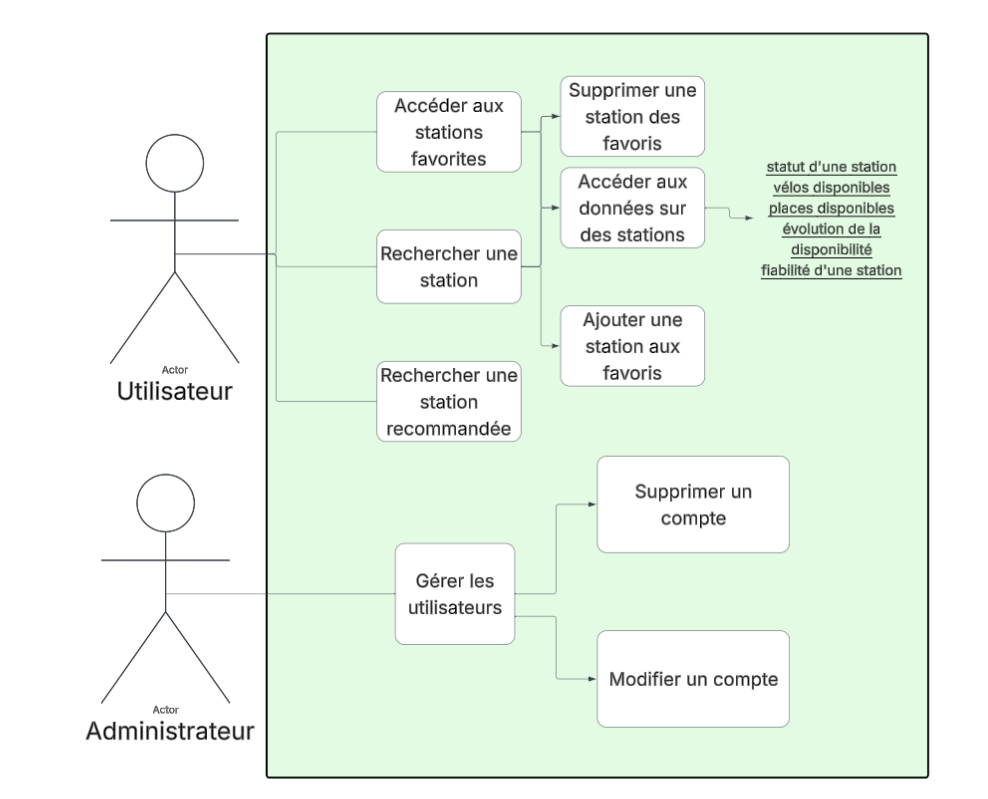
\includegraphics[keepaspectratio]{../ressources/Diagramme/Diagramme_cas_utilisation.png}}

}

\caption{Diagramme des cas d'utilisation}

\end{figure}%

~~~~~~~~ Deux profils d'utilisateurs existent sur l'application : le
profil utilisateur et le profil administrateur. Chacun doit créer puis
se connecter à un compte auquel est associée la fonction utilisateur ou
administrateur. Le compte administrateur permet de gérer les
utilisateurs, c'est-à-dire modifier leurs données ou supprimer des
comptes par exemple. Le compte utilisateur est celui qui donne accès au
plus grand nombre de fonctionnalités. Parmi les fonctionnalités
principales, un utilisateur peut rechercher une station afin d'accéder à
ses données et statistiques, ajouter une station à ses favoris pour que
son accès via l'application soit plus direct, plus largement gérer ses
stations favorites, et demander une suggestion de station en fonction de
sa fiabilité.

\subsubsection{Diagramme d'architecture}\label{diagramme-darchitecture}

~~~~ blablabla

\begin{figure}[H]

{\centering \pandocbounded{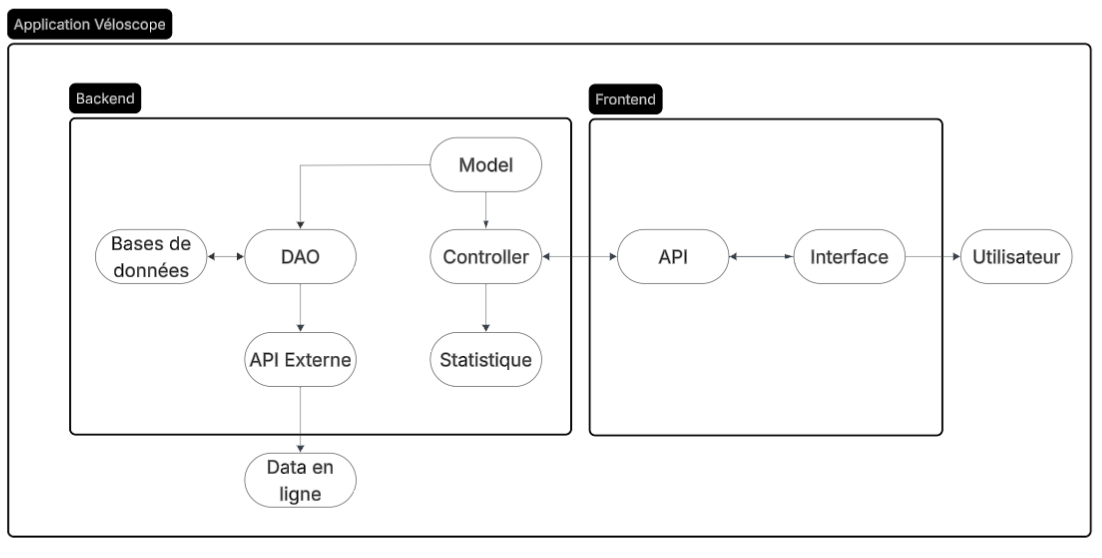
\includegraphics[keepaspectratio]{../ressources/Diagramme/Diagramme_architecture.png}}

}

\caption{Diagramme d'architecture}

\end{figure}%

~~~~ Le diagramme d'architecture présente les différentes composantes de
l'application Véloscope ainsi que le manière dont elles intéragissent
entre elles. Chacune répond à un rôle bien précis détaillé ci-dessous.
Nous retrouvons également les éléments avec lesquels l'application
communique : les utilisateurs et l'API externe.

L'utilisateur est extérieur à l'application. Il est à l'origine des
requêtes à laquelle elle doit pouvoir répondre. Lorsqu'il effectue une
demande, elle est reçu par le Controller. C'est le point d'entrée de
notre application. Cette demande est ensuite transmise à la partie
Analysis qui réalise l'ensemble des calculs nécessaires pour y répondre.
Elle calcule le taux de remplissage d'une station ou son score de
fiabilité.

La partie Model pemret de structurer les données utilisées par
l'application. Elle associe à chaque objet l'ensemble des informations
qui lui appartiennent. Une station dispose par exemple toujours d'un
identifiant, d'un nom, d'une capacité et une position géographique. Elle
est utilisé par le Parser et le Controller pour manipuler les données de
manière structurée.

Le DAO est la partie qui permet de lire et d'enregistrer les relevés
issus de l'API externe dans notre base de données. Avant que la DAO
puisse les enregistrer, les données de l'API externe passent par le
PARSER. Il les convertit dans un format recevable pour l'application. Ce
qui permet à la DAO de les stocker dans la base de données qui conserve
l'ensemble des informations nécessaires à l'utilisation et au
fonctionnement de l'application. Dans le cadre de notre projet, il
s'agit de PostgreSQL.

L'API externe est la base de données à partir de laquelle nous
recueillons les données nécessaire au développement de notre
application.

Finalement le fonctionnement de l'application est le suivant. Toutes les
15 minutes API externe envoie des information au Parser qui les
convertit. La DAO les enregistre et les stocke dans notre base de
données. Lorqu'un utilisateur effectue une requête qur l'application, le
controller reçoit sa demande et la trasnfère à la partie analysis qui
effectuent les calculs nécessaires pour y répondre.

\subsubsection{Diagramme d'activité}\label{diagramme-dactivituxe9}

~~~~ blablabla

\pandocbounded{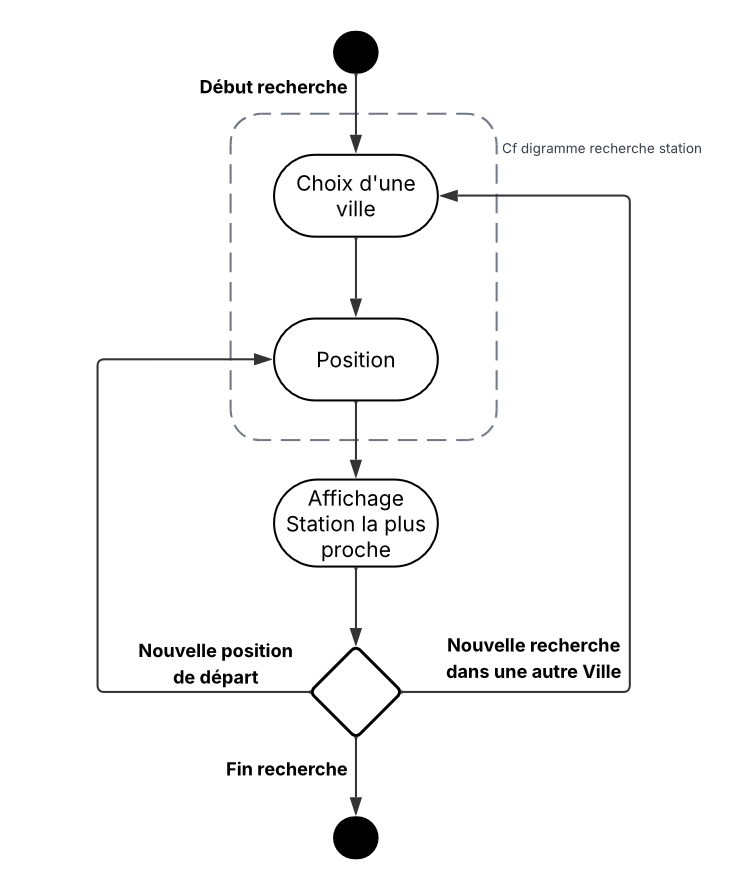
\includegraphics[keepaspectratio,alt={Diagramme d'activité préférences utilisateur}]{../ressources/Diagramme/Diagramme_activite_pref_utilisateur.png}}
~~~~ Ce diagramme d'activité représente les grandes étapes de la
recherche d'une station par l'utilisateur. Il commence par saisir le nom
d'une ville. En renseigant sa position, l'application lui renvoie la
station la plus proche. Si une station est trouvée, l'application
récupère les informations asscoiées les plus récentes. Il peut ensuite
lancer une nouvelle recherche au sein de la même ville, rechercher une
nouvelle ville ou mettre fin à ses recherches.

\begin{figure}[H]

{\centering \pandocbounded{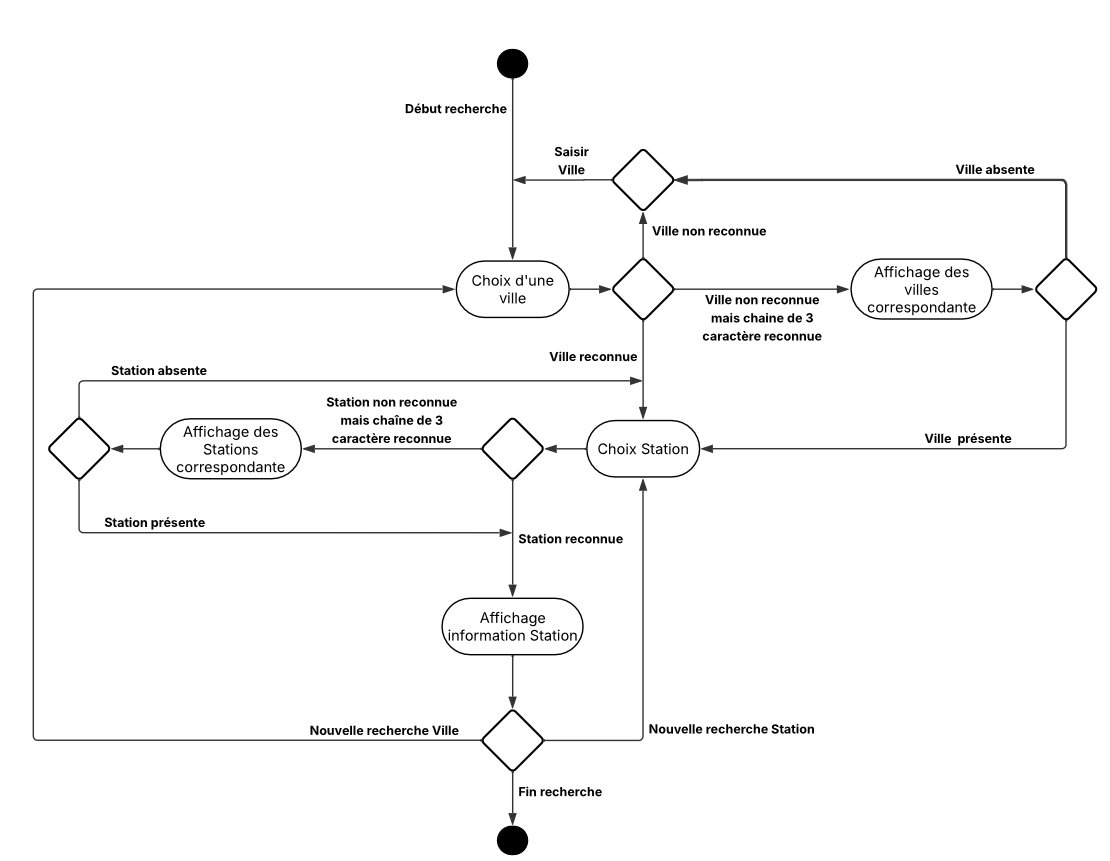
\includegraphics[keepaspectratio]{../ressources/Diagramme/Diagramme_activite_recherche_station.png}}

}

\caption{Diagramme d'activité recherche station}

\end{figure}%

Le diagramme d'activité ci-dessus est davantage détaillé. Lorsque
l'utilisateur recherche une ville, il est confronté à différentes
réponses de l'application. Dans le premier cas, la ville n'est pas
reconnue. L'utilisateur doit relancer une recherche? Si les trois
premiers caractères sont reconnus, l'application affiche la liste des
villes correspondantes. Si la ville recherchée y figure ou si la ville
avait été direcment reconnue, l'utilisateur peut choisir une station. Si
la station est reconnue, l'application affiche les informations
associées et la requête prend fin. De la même manière que pour les
villes, une chaîne de trois caractères permet d'afficher une liste de
stations correpondantes. Si la station recherchée n'apparaît pas,
l'utilisateur est invité à saisir un nom de station diffent. Si la
station est présente dans la liste, l'utilisateur la sélectionne et les
informations associées d'affichent. L'utilisateur peut mettre fin à sa
recherche, rechercher une autre ville ou une autre station.

\subsubsection{Modèle des données}\label{moduxe8le-des-donnuxe9es}

~~~~ blablabla

\begin{figure}[H]

{\centering \pandocbounded{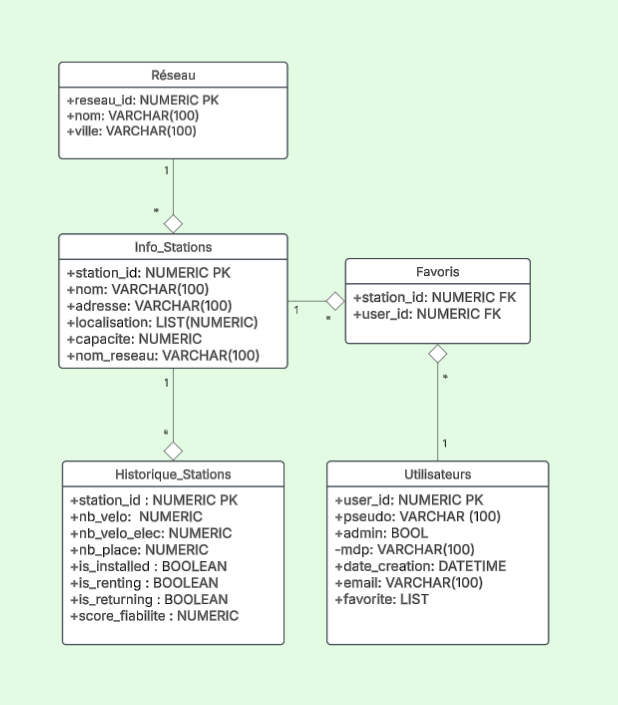
\includegraphics[keepaspectratio]{../ressources/Diagramme/Modele_donnees.png}}

}

\caption{Modèle de données}

\end{figure}%

~~~~ blablabla

\subsubsection{Diagramme de classes}\label{diagramme-de-classes}

\subsubsection{Diagrammes de séquence}\label{diagrammes-de-suxe9quence}

~~~~ blablabla

\begin{figure}[H]

{\centering \pandocbounded{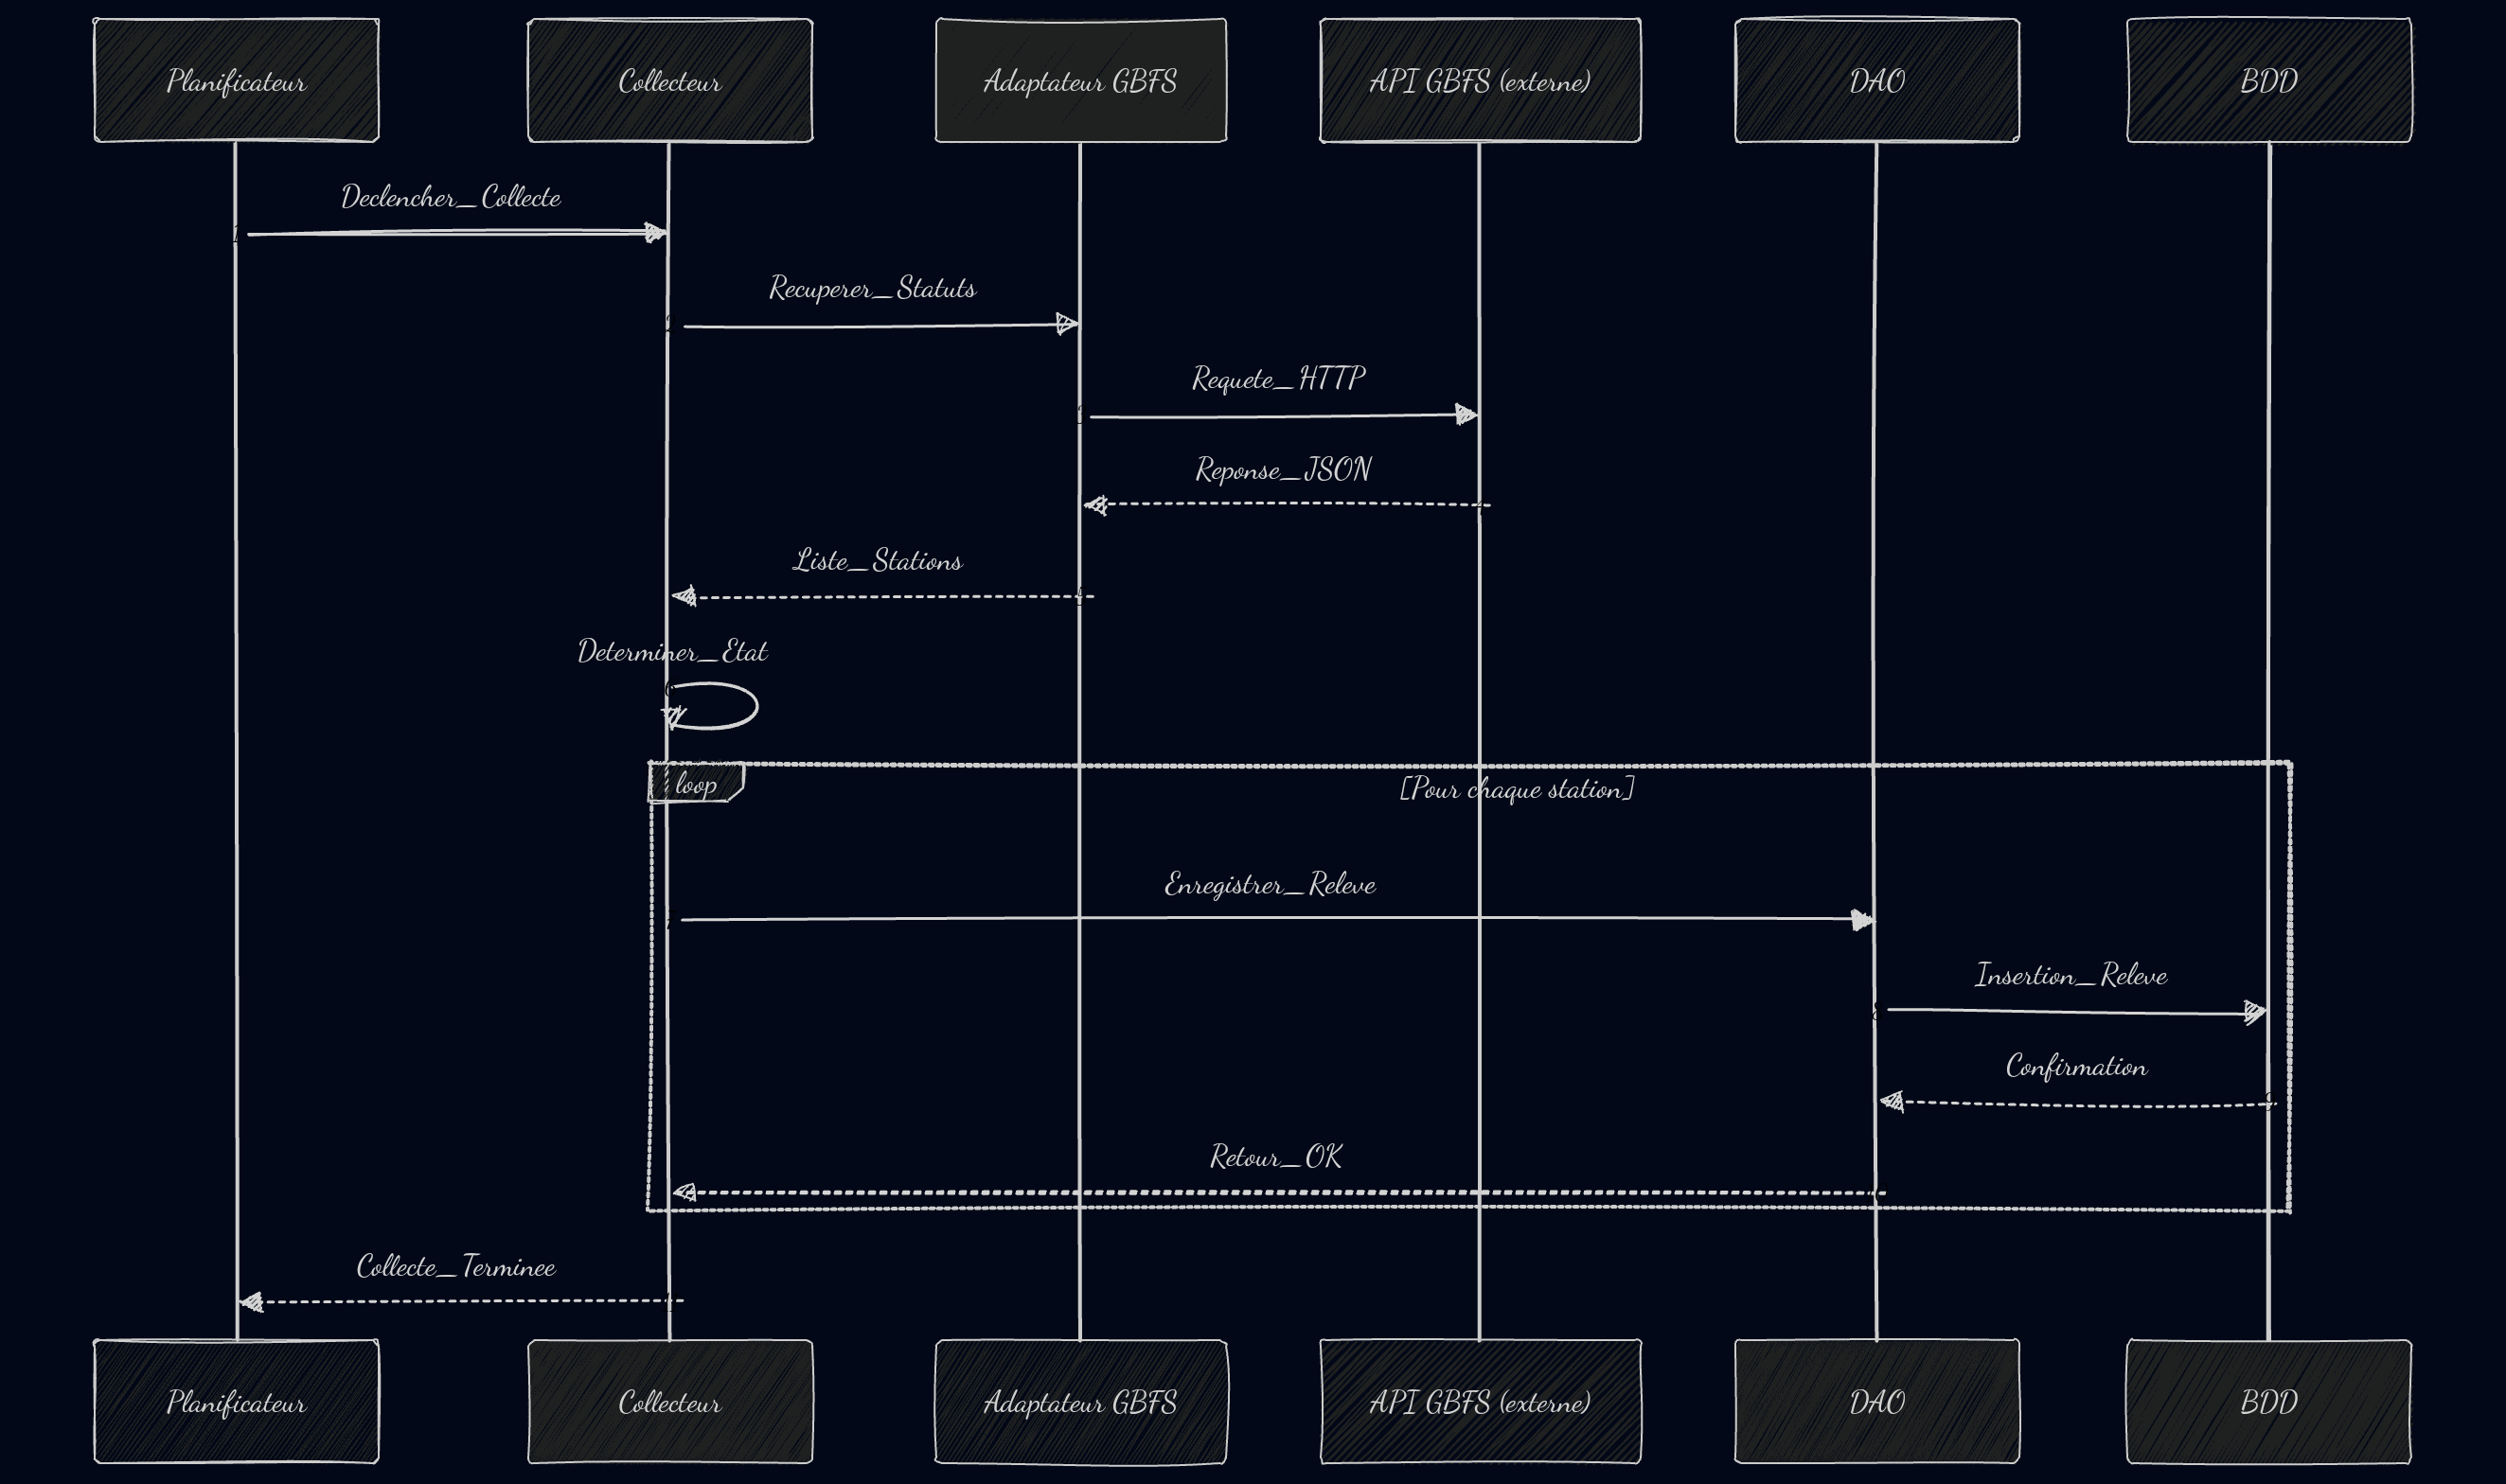
\includegraphics[keepaspectratio]{../ressources/Diagramme/Diagramme_sequence_collecte_donnees_F2.jpg}}

}

\caption{Diagramme de séquence pour la collecte de données}

\end{figure}%

~~~~ blablabla

\begin{figure}[H]

{\centering \pandocbounded{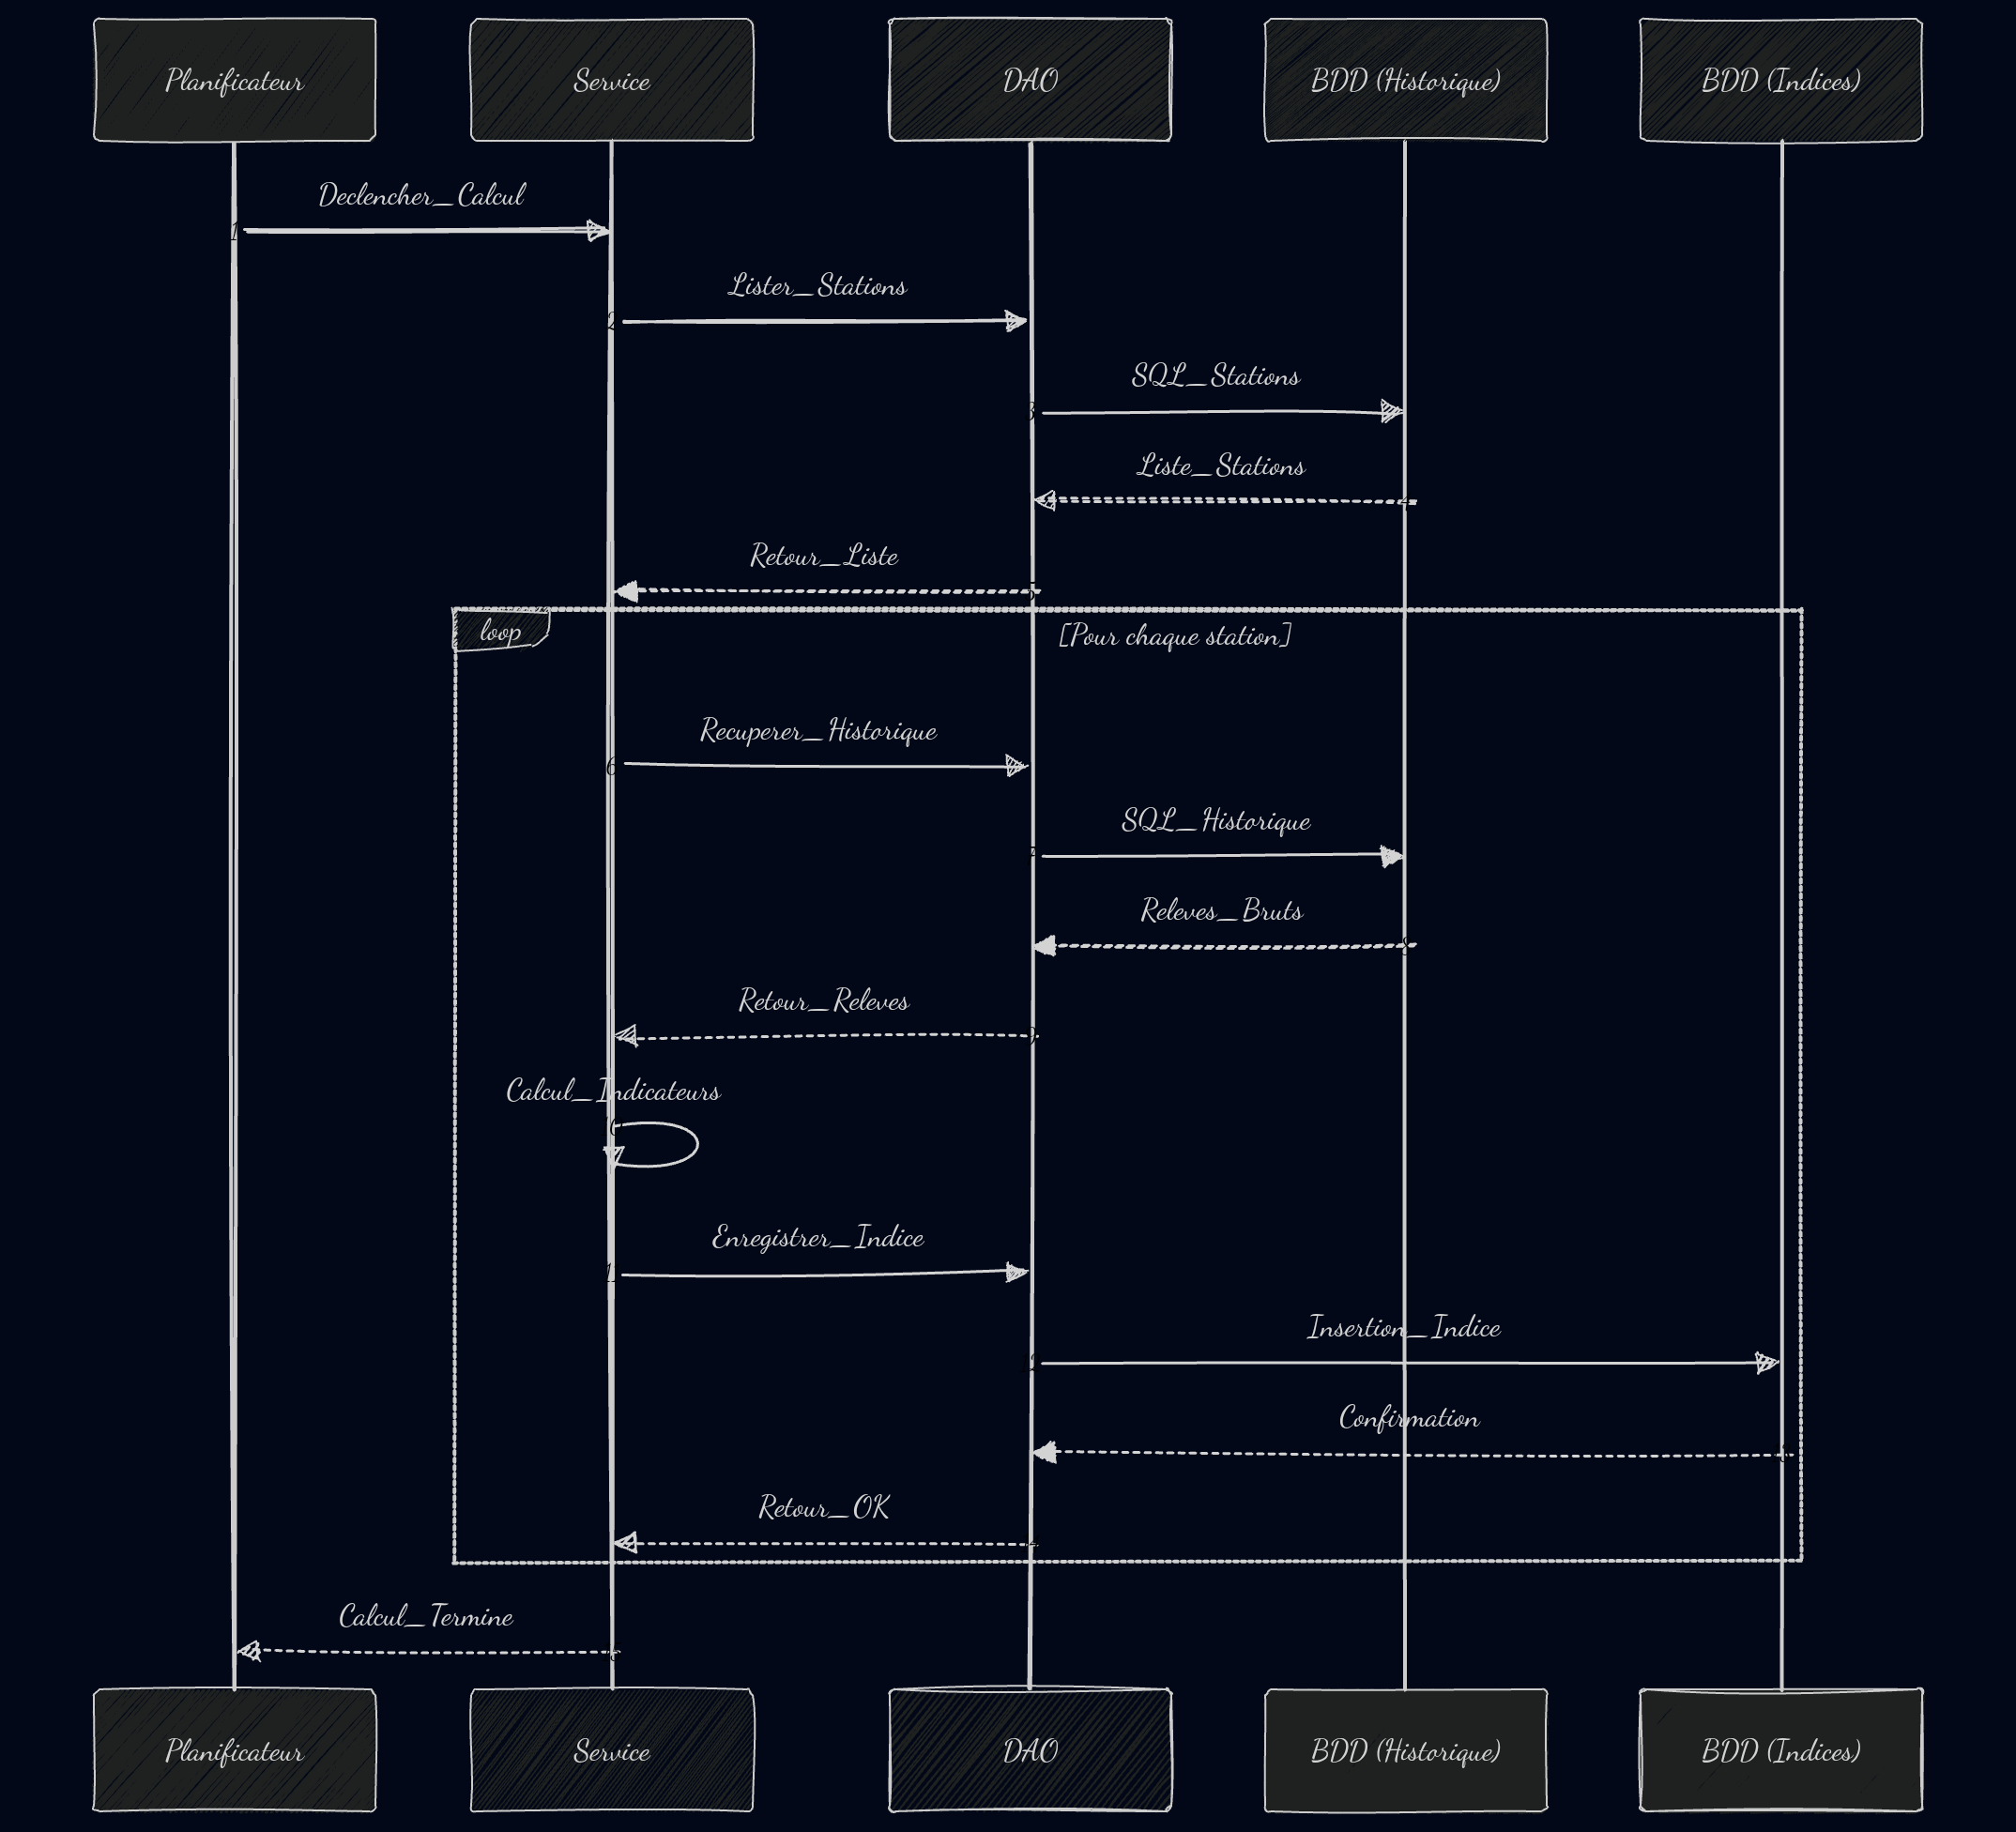
\includegraphics[keepaspectratio]{../ressources/Diagramme/Diagramme_sequence_score_fiabilite_F4.jpg}}

}

\caption{Diagramme de séquence pour le score de fiabilité}

\end{figure}%

~~~~ blablabla

\begin{figure}[H]

{\centering \pandocbounded{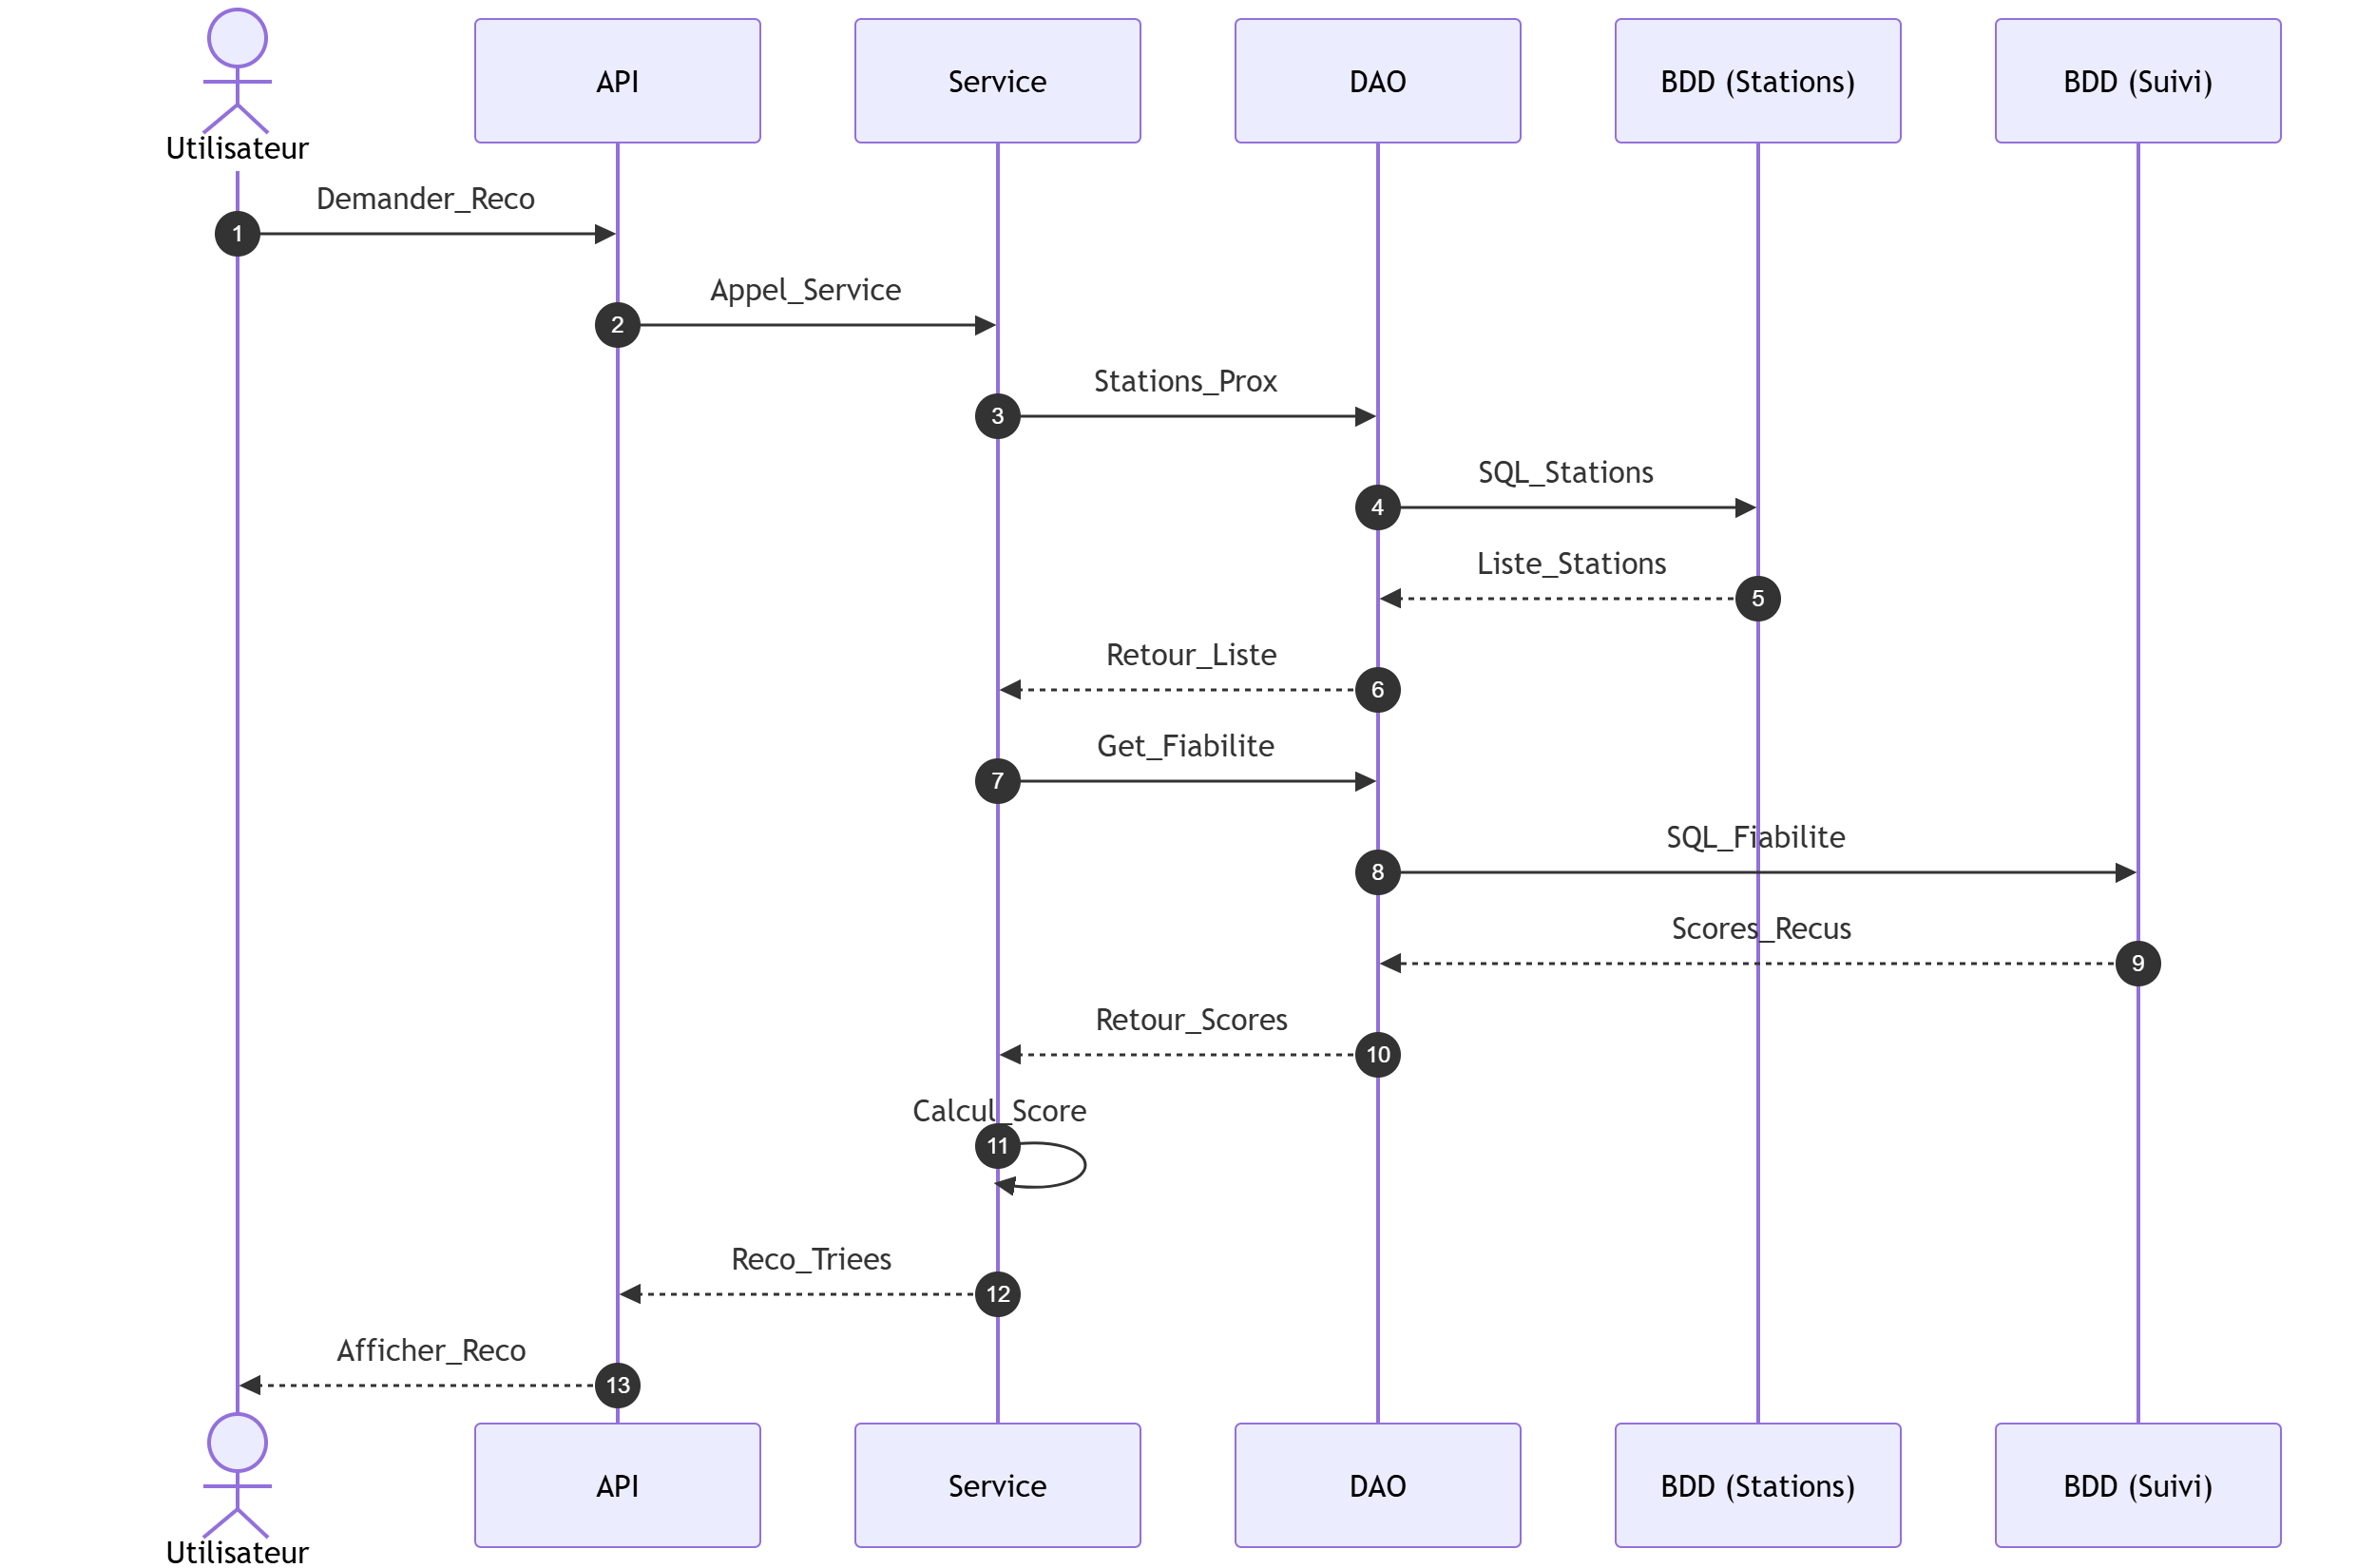
\includegraphics[keepaspectratio]{../ressources/Diagramme/Diagramme_sequence_reco_station_F5.png}}

}

\caption{Diagramme de séquence pour la recommandation de station}

\end{figure}%

~~~~ blablabla

\subsection{Fonctionnalités de
l'application}\label{fonctionnalituxe9s-de-lapplication}

~~~~~~~~ L'application vise à faciliter l'usage de réseaux de vélos en
libre-service en permettant à ses utilisateurs de voir clairement en
temps réel la disponibilité des stations et en l'eur proposant des
analyses de fiabilité des stations dans le temps'analysant dans le
temps. L'application a aussi vocation à proposer des recommandations de
stations aux utilisateurs en fonction de leurs besoins spécifiques et
des tendances observées à travers l'historique des stations.

\paragraph{La gestion des
utilisateurs}\label{la-gestion-des-utilisateurs}

~~~~~~~~ Chaque utilisateur peut se créer un compte personnel puis se
connecter à l'application. Une fois connecté à l'application,
l'utilisateur a accès à toutes es données et statistiques, et peut
enregistrer ses stations préférées comme favorites, ce qui lui permettra
d'y accéder plus rapidement. Certains utilisateurs sont aussi
administrateurs, ce qui leur permet de gérer les utilisateurs :
supprimer des comptes, réinitialiser les mots de passe, etc.

\paragraph{La collecte des données}\label{la-collecte-des-donnuxe9es}

~~~~~~~~ La collecte des données se fait à travers le DAO qui interroge
l'API toutes les 15 minutes pour en récupérer les données puis les
stocker dans une base PostgreSQL qui conservera un historique complet.
~~~~~~~~ Les informations récupérées par le DAO seront :

\begin{itemize}
\tightlist
\item
  le nom de la station
\item
  la date et l'heure de l'actualisation de l'API
\item
  le nombre de vélos disponibles
\item
  le nombre de places disponibles
\item
  le nombre de vélos électriques (disponibles ?)
\item
  l'état de la station
\end{itemize}

\paragraph{La consultation d'une
station}\label{la-consultation-dune-station}

~~~~~~~~ L'utilisateur peut rechercher une station et en consulter les
informations, dont :

\begin{itemize}
\tightlist
\item
  son état actuel
\item
  le nombre de vélos disponibles
\item
  sa capacité
\item
  son taux de remplissage
\item
  l'évolution de sa disponibilité sur une période choisie entre : les
  dernières 24 heures, les 7 derniers jours et le 30 derniers jours.
\end{itemize}

\paragraph{Le score de fiabilité}\label{le-score-de-fiabilituxe9}

~~~~~~~~ Cette fonctionnalité attribue à chaque station un score qui
reflète sa fiabilité dans le temps. ~~~~~~~~ Pour chaque appel de l'API,
un statut est accordé à la station : la station ets qualifiée de vide si
elle n'a plus de vélos disponibles, saturée si elle n'a plus de place
disponible, et fonctionnelle dans les autres cas. ~~~~~~~~ A partir de
ces données récoltées au fur et à mesure des actualisations de l'API,
l'application calcule le pourcentage de temps passé vide ou saturée, et
la durée moyenne des périodes de saturation ou de pérunie. A partir de
ces statistiques et de l'évolution du statut au cours du temps, un score
de fiabilité est calculé.

\paragraph{La recommandation de
station}\label{la-recommandation-de-station}

~~~~~~~~ L'application peut proposer des recommandations de stations à
chaque utilisateur en fonction :

\begin{itemize}
\tightlist
\item
  de la distance par rapport à l'utilisateur
\item
  de l'état actuel de la station (nombre de vélos disponibles,
  électriques ou non en fonction des préférences de l'utilisateur)
\item
  de la fiabilité historique de la station et de ses tendances récentes
\end{itemize}

\subsection{Présentation des menus}\label{pruxe9sentation-des-menus}

\subsection{Liste des principaux
composants}\label{liste-des-principaux-composants}




\end{document}
